\section{Simulation mit MATLAB}

%-------------------------------------------------------------------------------
%
% Aliasing
%
%-------------------------------------------------------------------------------
\subsection{Aliasing}
\subsubsection{Aufgabenstellung}
\begin{enumerate}
\item Wählen sie Frequenz und Abtastfrequenz so, dass eine Aliasingfrequenz von $440$Hz auftritt. Überprüfen sie das Resultat graphisch und akustisch (Klavier).
\item Erzeugen Sie einen Frequenzsweep, bei dessen Abtastung Aliasing auftritt. Wählen Sie als Anfangsfrequenz eine Frequenz im Hörfrequenzbereich, und als Endfrequenz eine Frequenz um $3 \cdot f_c$. \\
Überprüfen Sie das Resultat graphisch (sowohl im Zeitbereich als auch im Frequenzbereich) und akustisch. 
\item Wählen Sie die Datei ``Flöte'' aus. Durch Eingabe einer neuen Samplingfrequenz ($44100/L$, wobei $L$ ganzzahlig sein muss), kann das eingelesene Audiosignal ohne Bandbegrenzung unterabgetastet werden. Schätzen Sie die Auswirkungen ab. Überprüfen sie akustisch die Auswirkungen des Downsamplings ohne Einhaltung des Abtasttheorems. Ab welcher Frequenz werden Aliasing Effekte hörbar? Wodurch ergibt sich diese Frequenz? Ab welcher Frequenz werden Aliasingeffekte hörbar? Wodurch ergibt sich diese Frequenz?
\end{enumerate}



\subsubsection{Tabellen}

\subsubsection{Formeln}

\subsubsection{Berechnungsbeispiele}

\subsubsection{Diagramme}
\begin{figure}[h!]
\centering
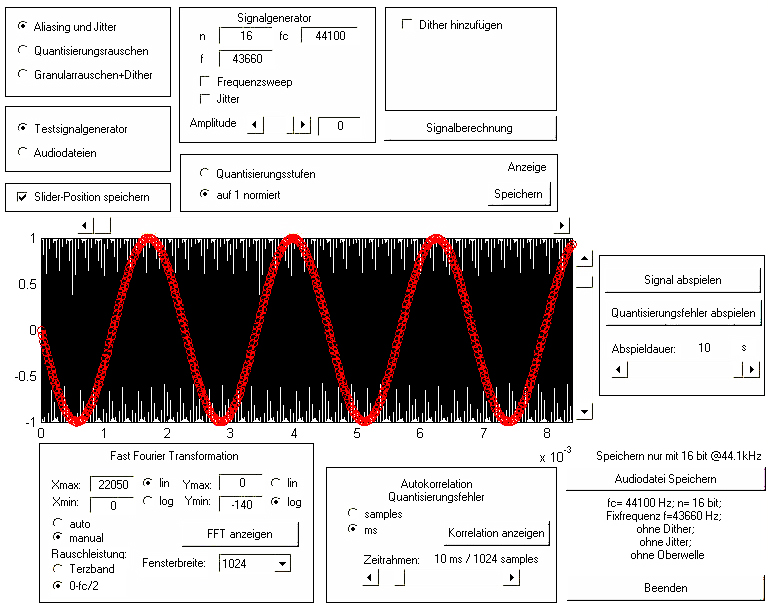
\includegraphics[width=\columnwidth]{figures/Aufg1/1_1.JPG} 
\caption{Test}
\end{figure}

\begin{figure}[h!]
\centering
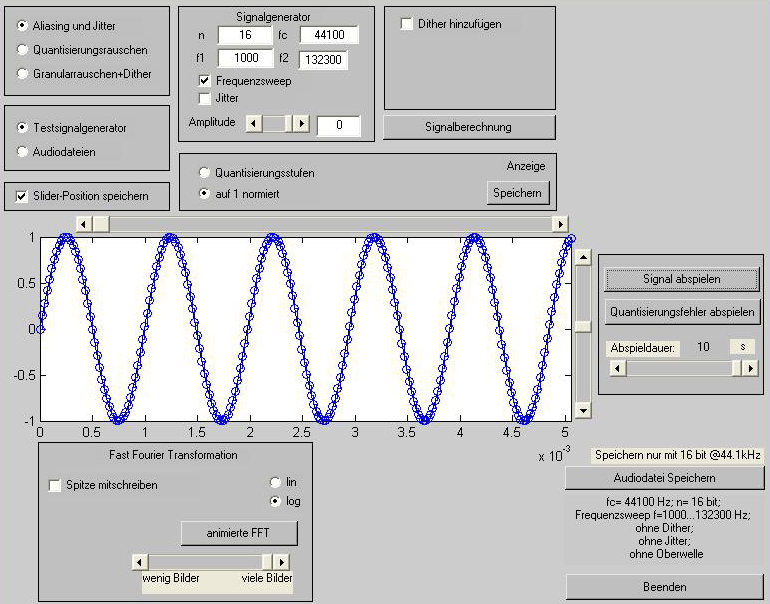
\includegraphics[width=\columnwidth]{figures/Aufg1/1_2.JPG} 
\caption{Test}
\end{figure}


\subsubsection{Diskussion}
\pagebreak

%-------------------------------------------------------------------------------
%
% Quantisierungsfehler, Leistungsdichtespektrum
%
%-------------------------------------------------------------------------------

\subsection{Quantisierungsfehler, Leistungsdichtespektrum}
\subsubsection{Aufgabenstellung}
\begin{enumerate}
\item Wie sieht der Quantisierungsfehler bei Vollaussteuerung und $8$ bit Wortbreite aus? In welchem Bereich liegt die Amplitude des Quantisierungsfehlers? Sind die Voraussetzungen für $SNR = 6.02 \cdot k$ erfüllt? Welche Charakteristik hat das Fehlersignal? Verwenden Sie das Simulationsprogramm zum Anzeigen des Quantisierungsfehlers in auf $1$ normierten Spannungswerten und Quantisierungsstufen. 
\item Berechnen Sie den erwarteten Signal-Rauschabstand (SNR) und die Quantisierungsrauschleistungs dichte für die gewählte Auflösung. Welchen Einfluss hat die FFT-Fensterbreite auf das Amplitudenspektrum bzw. die Leistungsdichteverteilung des Quantisierungsrauschens?
Überprüfen Sie den berechneten SNR und Quantisierungsrauschleistungsdichteverteilung bei verschiedenen FFT-Fensterbreiten mit dem Simulationsprogramm. 
\item Berechen Sie die Rauschleistung in einem Terzband und überprüfen Sie das Ergebnis mit dem Simulationsprogramm (empfohlene Wahl: $f_c = 48kHz, f_{Signal} = 890.625Hz$). 
\end{enumerate}



\subsubsection{Tabellen}

\subsubsection{Formeln}

\subsubsection{Berechnungsbeispiele}

\subsubsection{Diagramme}

\begin{figure}[h!]
\centering
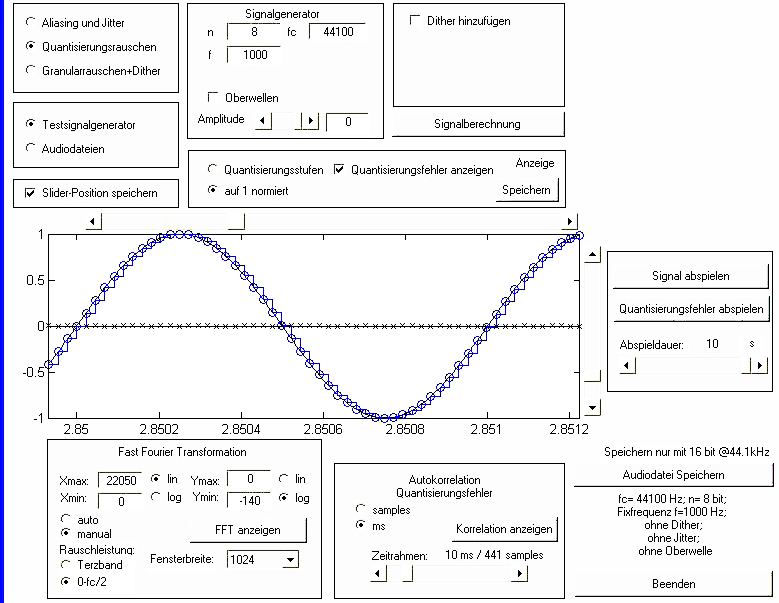
\includegraphics[width=\columnwidth]{figures/Aufg1/2_1_1.JPG} 
\caption{Test}
\end{figure}

\begin{figure}[h!]
\centering
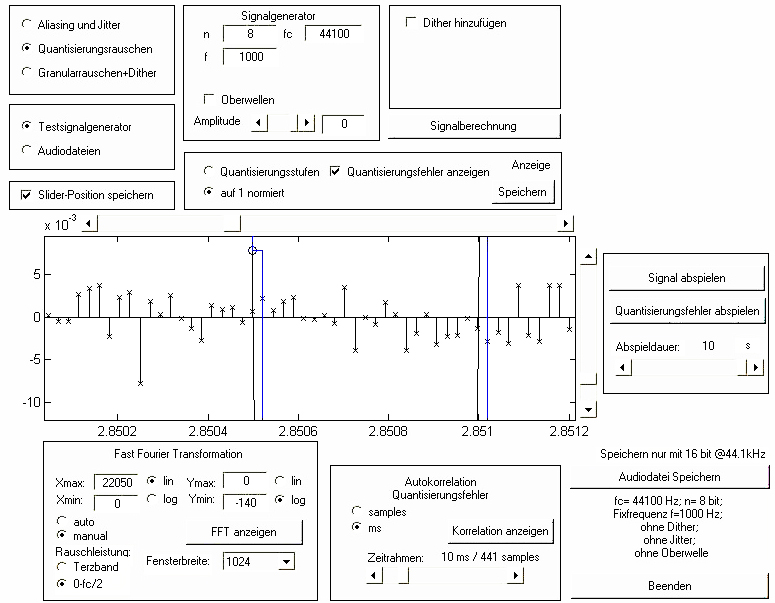
\includegraphics[width=\columnwidth]{figures/Aufg1/2_1_3.JPG} 
\caption{Test}
\end{figure}

\begin{figure}[h!]
\centering
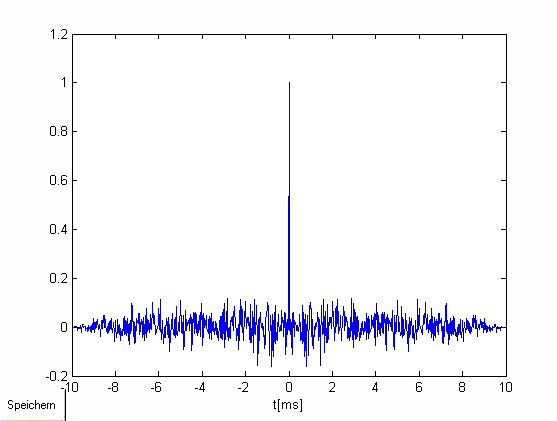
\includegraphics[width=\columnwidth]{figures/Aufg1/2_1_korr.JPG} 
\caption{Test}
\end{figure}

\begin{figure}[h!]
\centering
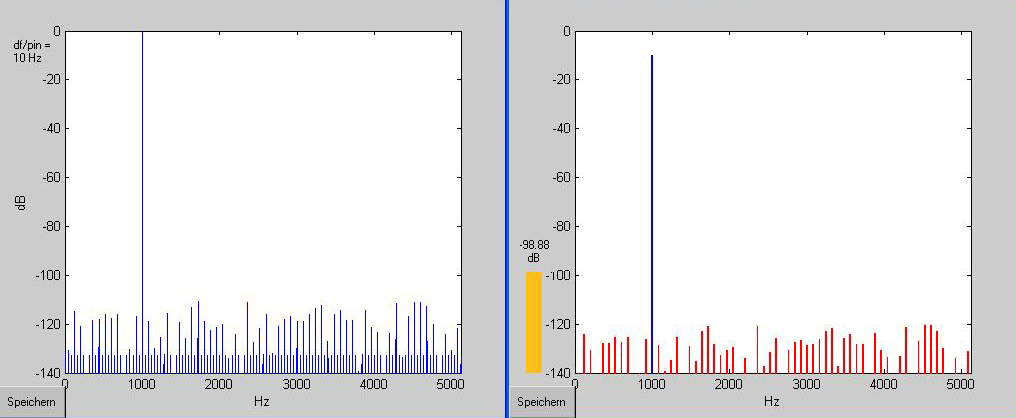
\includegraphics[width=\columnwidth]{figures/Aufg1/2_2_fenster_ok.JPG} 
\caption{Test}
\end{figure}

\begin{figure}[h!]
\centering
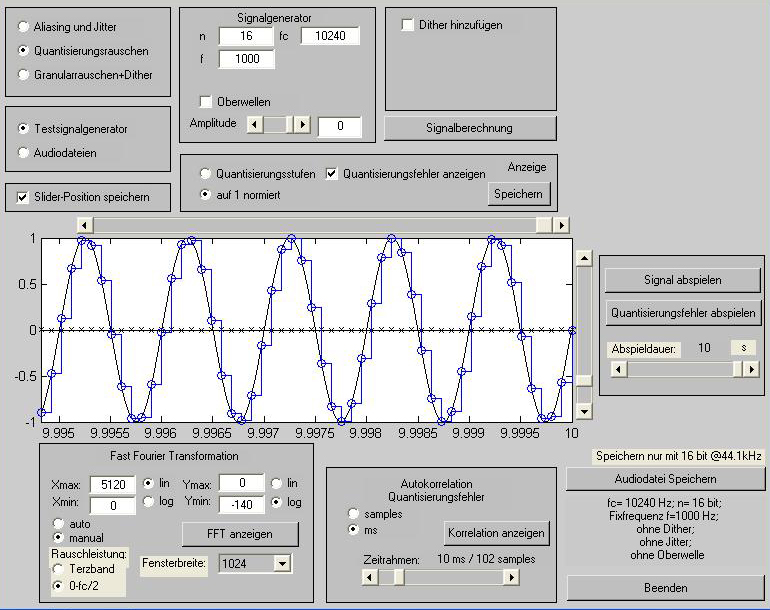
\includegraphics[width=\columnwidth]{figures/Aufg1/2_2_fenster_ok_einstell.JPG} 
\caption{Test}
\end{figure}

\begin{figure}[h!]
\centering
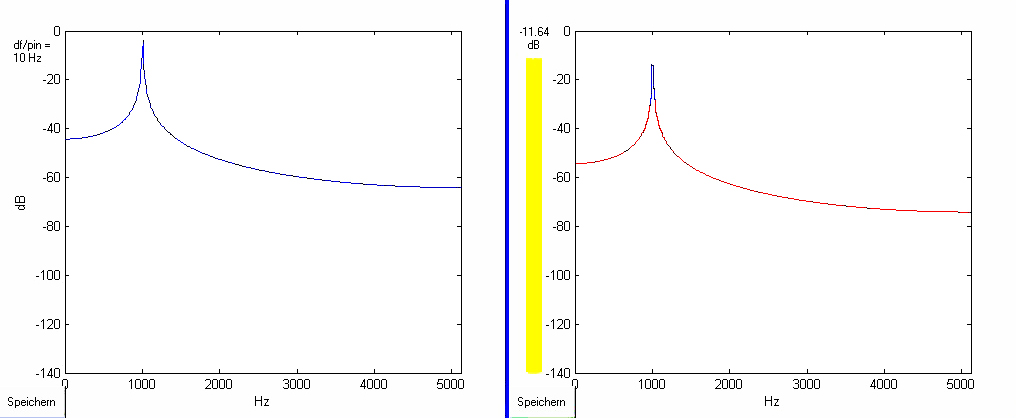
\includegraphics[width=\columnwidth]{figures/Aufg1/2_2_fenster_schlecht.JPG} 
\caption{Test}
\end{figure}

\begin{figure}[h!]
\centering
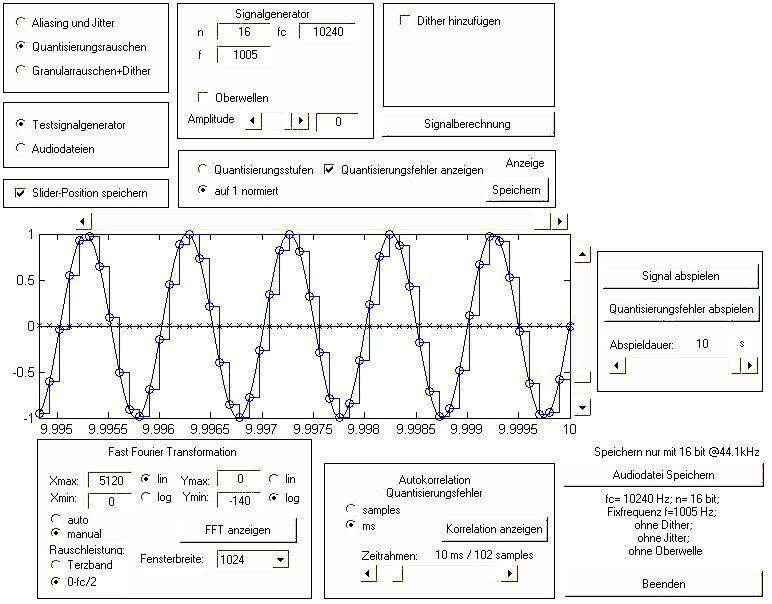
\includegraphics[width=\columnwidth]{figures/Aufg1/2_2_fenster_schlecht_einstell.JPG} 
\caption{Test}
\end{figure}

\begin{figure}[h!]
\centering
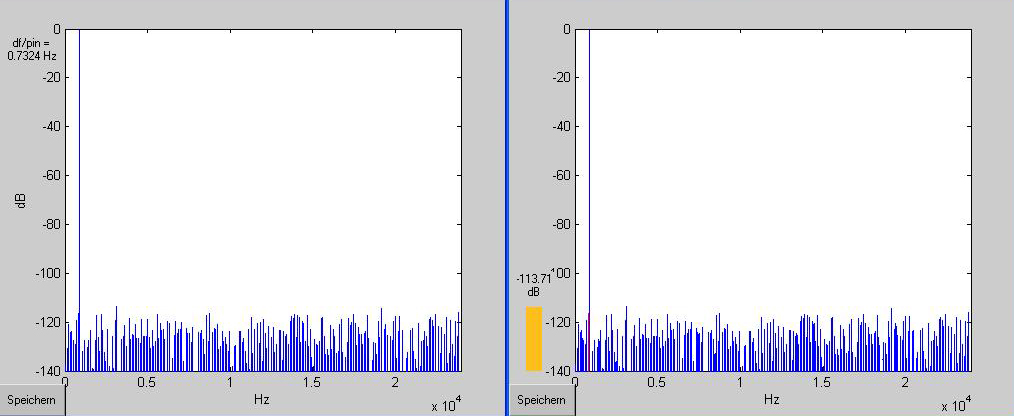
\includegraphics[width=\columnwidth]{figures/Aufg1/2_3_890hz.JPG} 
\caption{Test}
\end{figure}

\subsubsection{Diskussion}

%-------------------------------------------------------------------------------
%
% Granularrauschen und Dither
%
%-------------------------------------------------------------------------------

\subsection{Granularrauschen und Dither}
Diese Unterübung wurde aus Zeitgründen nur mündlich mit dem Laborbetreuer erarbeitet. 

\subsection{Geräteliste}